\documentclass[12pt]{article}
\usepackage{sbc-template}
\usepackage{graphicx,url}
\usepackage[utf8]{inputenc}
\usepackage[brazil]{babel}
\usepackage[latin1]{inputenc}     
\usepackage{amsmath}
\sloppy


\title{Heurísticas e Busca Exata para o Problema de Bin Packing}

\author{Leandro A. De Araujo\inst{1}, Daniel C. Dos Santos\inst{1}}

\address{Departamento de Informática e Matemática Aplicada (DIMAp) \\
  Universidade Federal do Rio Grande do Norte (UFRN)
  \email{leandro.andrade.401@ufrn.edu.br, daniel.coelho.708@ufrn.edu.br}
}
\begin{document} 

\maketitle

\begin{abstract}
This work compares four heuristics for the bin packing problem with two exact methods: Branch and Bound and a randomized Las Vegas variant. Experiments on 40 OR-Library instances showed mean excesses of 1.00 and 0.98 bins for the repacking heuristics at capacities 150 and 176, respectively. At capacity 150, the exact methods achieved a mean excess of 0.70 bins and proved optimality in 12 instances.
\end{abstract}

\begin{resumo}
Este trabalho compara quatro heurísticas para o problema do \textit{bin packing} com dois métodos exatos: Branch and Bound e uma variante aleatorizada Las Vegas. Nos experimentos com 40 instâncias da OR-Library, as heurísticas com remanejamento tiveram excesso médio de 1,00 e 0,98 bin nas capacidades 150 e 176, respectivamente. Na capacidade 150, os métodos exatos obtiveram excesso médio de 0,70 bin e comprovaram a otimalidade em 12 instâncias.
\end{resumo}

\section{Introdução}

O \textit{Bin Packing} (ou Problema de Empacotamento em Caixas) consiste em um problema clássico de otimização matemática e computacional, cujo objetivo é acomodar um conjunto de itens de tamanhos diferentes no menor número possível de \textit{bins} (caixas). O problema possui diversas aplicações práticas, como na logística, na indústria e na alocação de memória computacional \cite{ambrose2025}.

Nesse contexto, cada item possui uma medida diferente. No modelo mais clássico do problema, todos os bins possuem a mesma capacidade máxima, mas existem variações importantes que permitem caixas com capacidades distintas. O objetivo é encontrar o menor número de bins necessários para guardar todos os itens, sem deixar nenhum de fora e respeitando o limite de cada caixa.

Como o problema é computacionalmente difícil, heurísticas construtivas são úteis para produzir soluções viáveis em tempo prático \cite{ambrose2025}. Este trabalho implementa e analisa quatro estratégias: First Fit (FF), First Fit Decreasing com uma etapa adicional de remanejamento (FFDR), Best Fit e Best Fit Decreasing com uma etapa adicional de remanejamento (BFDR).

Como o problema é computacionalmente difícil, heurísticas construtivas são úteis para produzir soluções viáveis em tempo prático \cite{ambrose2025}. Na primeira unidade, este trabalho implementou e analisou quatro estratégias: First Fit (FF), First Fit Decreasing com remanejamento (FFDR), Best Fit (BF) e Best Fit Decreasing com remanejamento (BFDR). Dando continuidade ao projeto, na segunda unidade também foi implementado um algoritmo exato baseado em Branch and Bound, cujos resultados são comparados aos das quatro heurísticas já estudadas. Além disso, é analisada uma variação aleatorizada do Branch and Bound, denominada Las Vegas.

\section{Descrição Matemática e Complexidade}

A descrição matemática do problema clássico é: sejam $n$ itens com tamanhos positivos $t_1,\ldots,t_n$ e caixas idênticas de capacidade $C$. Deve-se atribuir cada item a exatamente uma caixa, respeitando, para toda caixa $j$, a restrição
\begin{equation}
  \sum_{i\in B_j} t_i \leq C,
\end{equation}
em que $B_j$ representa o conjunto de itens atribuídos à caixa $j$, e minimizando o número de caixas não vazias \cite{ambrose2025}.

Neste projeto, cada instância fornece a capacidade das caixas, a quantidade de itens, os tamanhos dos itens e uma referência da melhor solução conhecida.

Quanto à complexidade, o Bin Packing é classificado como um problema NP-difícil em sua versão de otimização, enquanto o problema de decisão é classificado como NP-completo. Este último pergunta se os itens podem ser acomodados em no máximo $k$ caixas. A demonstração de que este problema de decisão é realmente NP-completo é feita por Ambrose \cite{ambrose2025} por meio de uma redução do problema de Emparelhamento Tridimensional (\textit{Three-Dimensional Matching}).

Sendo assim, não se conhece até hoje um algoritmo polinomial que encontre sempre a solução ótima do problema. A existência de um algoritmo desse tipo implicaria que $P=NP$.

\subsection{Estado da Arte em Algoritmos Exatos}

Entre os métodos exatos para o Bin Packing estão os algoritmos baseados em Branch and Bound. Korf (2002) descreve o método clássico de Martello e Toth, que processa os itens em ordem decrescente e ramifica entre as possibilidades de colocá-los nos bins existentes ou abrir novos bins. O artigo também apresenta o \textit{Bin Completion}, que explora diferentes formas de completar um bin, em vez de decidir a cada etapa onde colocar o próximo item \cite{korf2002}.

Fukunaga e Korf (2007) desenvolvem melhorias para o \textit{Bin Completion} e o aplicam a diferentes problemas de empacotamento e cobertura. Para o Bin Packing clássico, os autores relatam que a abordagem não foi competitiva com os métodos baseados em \textit{cutting stock} considerados no estudo \cite{fukunaga2007}. Neste projeto, foi implementada uma busca item a item baseada em Branch and Bound, e não o \textit{Bin Completion}.

\section{Heurísticas e Implementação}

Neste projeto, foram implementadas quarto heurísticas para o problema de empacotamento em caixas: First Fit, First Fit Decreasing, Best Fit e  Best Fit Decreasing. A lógica fundamental para a construção desses algoritmos foi extraída das demonstrações passo a passo discutidas em \cite{video_youtube}, que ilustram de forma prática a mecânica de preenchimento dos bins. Essas estratégias foram posteriormente refinadas com base na literatura formal \cite{ambrose2025, friesen1986}. O código foi implementado utilizando a linguagem de programação C++.

\subsection{First Fit}

O First Fit (FF) é um algoritmo guloso que processa os itens na ordem recebida. Sendo assim, trata-se de um algoritmo \textit{online}, pois não precisa conhecer antecipadamente os próximos itens para realizar o empacotamento \cite{ambrose2025}. 

Para cada item, o algoritmo percorre todas as caixas já abertas até então e encaixa o item na primeira em que couber. Se não couber em nenhuma, ele cria/abre uma nova caixa. 

\subsection{First Fit Decreasing Com Remanejamento}

O First Fit Decreasing (FFD) é bem parecido com o First Fit, tendo como principal diferença o fato de ser um algoritmo \textit{offline}, por conhecer com antecedência todos os itens a serem organizados. A estratégia consiste em primeiro ordenar os itens em ordem não crescente de tamanho e, só então, aplicar a estratégia do First Fit \cite{ambrose2025}.

Essa ordenação visa realizar primeiro o posicionamento dos itens maiores, reduzindo assim a possibilidade de que eles fiquem sem espaço nas caixas já abertas.

No entanto, a versão implementada no nosso trabalho ainda possui uma etapa adicional: o remanejamento. Depois da primeira solução produzida pelo First Fit Decreasing, o algoritmo tenta remover caixas, ordenando-as pelo espaço restante em ordem decrescente. Para cada caixa candidata, tenta transferir seus itens, também em ordem decrescente de tamanho, para as outras caixas, utilizando novamente a estratégia First Fit. Uma remoção é aceita somente se todos os itens da caixa candidata puderem ser acomodados nas demais caixas, sem ultrapassar suas capacidades.

A utilização de estratégias como essa, de reorganização do conteúdo das caixas, também aparece na literatura. Friesen e Langston \cite{friesen1986}, por exemplo, investigam algoritmos que utilizam etapas de reorganização e transferência de itens para melhorar o empacotamento. Entretanto, o trabalho dos autores considera uma variante do problema com caixas de capacidades diferentes, enquanto nossa implementação utiliza caixas de capacidade fixa.

O objetivo do remanejamento implementado neste projeto é reduzir o número de caixas utilizadas, mantendo ainda uma solução válida. O algoritmo repete essa etapa de busca enquanto conseguir eliminar caixas.

\subsection{Best Fit}

 O Best Fit (BF) é um algoritmo guloso para o problema do bin packing. Diferente do First Fit, que insere o item na primeira caixa em que couber, o BF insere o item na caixa cuja soma com o novo item seja a maior possível (deixando o menor espaço residual).

Para cada item, o algoritmo percorre todas as caixas já abertas até então e encaixa o item na caixa com a menor sobra de espaço possível. Se não couber em nenhuma, ele abre uma nova caixa.

\subsection{Best Fit Decreasing com Remanejamento}
O  Best Fit Decreasing com Remanejamento (BFDR) é uma versão aprimorada do Best Fit original. Utilizando a mesma premissa de minimização do espaço residual, o BFD incorpora ordenação e busca local para alcançar uma solução de melhor qualidade.

Primeiramente, é realizada a ordenação do conjunto de itens em ordem decrescente, estratégia adotada para favorecer uma melhor ocupação das caixas. Em seguida, aplica-se o algoritmo \textit{Best Fit} padrão. Após essa etapa, tenta-se eliminar caixas por meio da realocação dos itens de uma caixa candidata para as demais, visando diminuir a quantidade total de caixas utilizadas no empacotamento.

\section{Análise das Heurísticas Implementadas}

\subsection{Complexidade de Tempo e Espaço}
Seja $n$ o número de itens e $m$ o número de bins abertos durante a execução. No \textbf{First Fit}, cada item pode exigir uma busca por todos os bins já abertos, com custo de até $O(m)$. Como essa busca é feita para cada um dos $n$ itens, o custo total é $O(nm)$. Como $m \leq n$, o pior caso da implementação direta utilizada é $O(n^2)$.

O \textbf{Best Fit} também percorre os bins abertos a cada inserção, mas escolhe aquele que ficará com a menor capacidade restante. Como a implementação usa uma busca linear para encontrar esse bin, o custo por item é $O(m)$, e o custo total é $O(nm)$, ou $O(n^2)$ no pior caso.

\textbf{First Fit Decreasing} (FFD) e \textbf{Best Fit Decreasing} (BFD) acrescentam uma ordenação dos itens em ordem não crescente, que custa $O(n\log n)$. Depois da ordenação, a construção inicial da solução ainda pode exigir até $O(n^2)$ operações de inserção. Portanto, sem considerar o remanejamento, o custo total dessas variantes é $O(n^2)$, pois esse termo domina o custo da ordenação.

Já nas variantes com \textbf{remanejamento}, o algoritmo tenta eliminar caixas realocando seus itens nas demais. Em uma rodada com $q$ caixas, podem ser testadas até $q$ candidatas. Como cada caixa candidata contém um grupo distinto de itens, ao longo da rodada são realocados no máximo $n$ itens. As cópias da solução e as buscas por espaço custam, juntas, $O(nq)$. No FFD com esta etapa adicional, a ordenação dos itens das candidatas acrescenta até $O(n\log n)$ por rodada.

Após cada eliminação bem-sucedida, o número de caixas diminui. Assim, com $M$ caixas ao final da construção inicial, o custo total do remanejamento é limitado por $O(nM^2+nM\log n)$. Como $M\leq n$, o limite no pior caso é $O(n^3)$ para ambas as variantes (esse custo já domina a ordenação e a construção inicial, que custam até $O(n^2)$).

O espaço utilizado é $O(n)$, pois a solução e as cópias temporárias armazenam, no máximo, os $n$ itens. Vale destacar que esta análise considera a implementação feita neste projeto, outras implementações dessas heurísticas podem ter custos diferentes.

\subsection{Garantias  de Aproximação}

A revisão de Ambrose (2025) apresenta limites assintóticos de $1{,}7$ para First Fit e Best Fit, e de $11/9$ para suas variantes decrescentes. No código deste projeto, o remanejamento só aceita uma configuração viável que use menos caixas do que a solução inicial. Assim, FFD+R e BFD+R não usam mais caixas que FFD e BFD, respectivamente, e herdam esses limites.

\section{Algoritmos Exatos}

\subsection{Branch and Bound}

O Branch and Bound foi usado para resolver o bin packing de forma exata. A ideia é montar a solução item por item, testando as possibilidades, e descartar os caminhos que não podem dar um resultado melhor do que o já encontrado. A busca vai até o fundo de um caminho antes de voltar e tentar outro, e os itens são tratados do maior para o menor. Essa estratégia de busca por atribuições de itens também é discutida para o Bin Packing por Korf \cite{korf2002}.

\subsubsection{Estratégia e Implementação}

Cada nó da busca é um empacotamento parcial. O algoritmo pega o próximo item e cria uma opção para cada lugar onde ele cabe: em cada bin já aberto que ainda tem espaço, e, quando isso ainda pode melhorar a solução conhecida, em um bin novo. Assim, cada nível da busca fixa o item em uma posição, e os níveis de baixo cuidam dos itens restantes. Desse jeito, o algoritmo considera, aos poucos, as formas de distribuir os itens que ainda podem melhorar a solução, sem precisar listar todas de uma vez.

Para reduzir o tamanho da busca, usam-se algumas estratégias. Primeiro, os itens são tratados do maior para o menor, o que costuma achar boas soluções logo no começo. Segundo, bins vazios são todos iguais entre si: quando é preciso abrir um bin novo, basta considerar um único bin vazio, porque testar vários bins vazios iguais daria a mesma solução e só aumentaria a busca. O algoritmo também trata como equivalentes os bins abertos que têm a mesma capacidade restante.

Durante a busca, o algoritmo guarda a melhor solução encontrada até o momento, que começa com uma solução obtida por uma heurística Best Fit Decreasing com remanejamento. Também são testadas permutações dos itens para tentar melhorar essa solução. No fim, a geração da tabela confere se todos os itens foram colocados exatamente uma vez e se nenhum bin passou da capacidade.

\subsubsection{Limites Inferiores e Podas}

O limite inferior global é o menor número possível de bins, dado por \(\lceil \text{soma dos itens} / \text{capacidade} \rceil\). Em cada nó, o algoritmo também calcula limites inferiores para os itens que ainda faltam, considerando o espaço livre nos bins abertos, os itens maiores que metade da capacidade e a quantidade de itens acima de outros limiares de tamanho.

Se o número de bins já abertos ou o limite inferior calculado não for menor do que a melhor solução já conhecida, aquele caminho é abandonado, porque continuar por ele não pode dar um resultado melhor. O tempo máximo também serve para parar a busca: se ela termina sem interrupção, a solução é ótima; se o tempo acaba antes, a solução é apenas a melhor encontrada até ali.

\subsubsection{Prova de Correção}

A correção do algoritmo se apoia em quatro pontos: toda solução construída respeita a capacidade dos bins; a busca testa todas as posições válidas para cada item, considerando apenas uma vez bins equivalentes; as podas são seguras, pois só cortam caminhos que não podem ser melhores que a solução atual; e, no fim, o algoritmo confere se os itens empacotados são exatamente os mesmos da instância. Assim, se a busca termina dentro do tempo, o resultado é ótimo; se o tempo acaba antes, o resultado é a melhor solução viável encontrada até aquele momento.

\subsubsection{Complexidade e Limite de Execução}

Se \(T\) representa o número de nós visitados, o trabalho realizado em cada nó pode custar até \(O(n\log n)\), devido ao cálculo dos limites inferiores e à ordenação dos bins candidatos. Como \(T\) pode crescer exponencialmente com o número de itens, o pior caso do algoritmo também é exponencial.

O espaço auxiliar pode chegar a \(O(n^2)\), pois a implementação mantém vetores de candidatos e capacidades restantes por nível da busca.

\subsection{Las Vegas: Variação Aleatorizada do Branch and Bound}

Os algoritmos Las Vegas são algoritmos probabilísticos que utilizam escolhas aleatórias durante a execução, mas não fornecem uma resposta incorreta. Essas escolhas podem alterar o caminho percorrido e o tempo de execução, enquanto a correção da resposta é preservada quando o algoritmo termina \cite{figueiredo2007}.

Neste trabalho, o Las Vegas é implementado como uma variação aleatorizada do Branch and Bound. Ele mantém a estrutura da busca e as regras de poda do algoritmo original, mas altera a ordem em que os bins candidatos são testados.

\subsubsection{Alterações em relação ao Branch and Bound}

Como explicado na subseção anterior, o Las Vegas mantém a estrutura de busca do Branch and Bound. A principal alteração é a ordem em que os bins candidatos são testados: eles são embaralhados em vez de seguirem uma ordem fixa.

A versão original do Branch and Bound também testa permutações para tentar melhorar a solução inicial, mas usa um valor inicial fixo para controlar essa aleatoriedade. No Las Vegas, um gerador pseudoaleatório controla tanto essas permutações quanto o embaralhamento dos candidatos. O valor inicial do gerador é definido no começo da execução e registrado nos resultados para identificar a sequência utilizada.

O embaralhamento não elimina alternativas, apenas muda a ordem da busca. Por isso, execuções diferentes podem levar tempos diferentes, mas, se a busca terminar, a solução ótima continua sendo comprovada. Essa variação no tempo, sem alterar a correção da resposta, caracteriza o paradigma Las Vegas \cite{figueiredo2007}.

\subsubsection{Garantia de correção}

Como o Las Vegas mantém as mesmas ramificações e podas do Branch and Bound, a prova de correção apresentada anteriormente também se aplica a ele. Sendo assim, por o embaralhamento não descartar alternativas, se a busca terminar, a solução ótima estará comprovada.

Na geração das tabelas, porém, a busca pode ser interrompida pelo limite de tempo. Nesse caso, o programa retorna uma configuração viável, mas registra que a otimalidade não foi comprovada.

\subsubsection{Complexidade e limite de execução}

O Las Vegas mantém a mesma complexidade assintótica do Branch and Bound, com pior caso exponencial. A ordem aleatória pode alterar a quantidade de nós visitados, mas não muda esse pior caso. Na geração dos resultados para este relatório, o limite configurado foi de 1200 segundos por instância.

\section{Instâncias Utilizadas}

Para avaliar as heurísticas que implementamos, foram utilizadas instâncias do problema de Bin Packing disponibilizadas pela OR-Library, uma biblioteca de conjuntos de testes para diferentes problemas de otimização. As instâncias utilizadas foram originalmente fornecidas por E. Falkenauer, em 1994, e estão disponíveis na biblioteca \cite{orlibrary}.

Neste projeto, foram utilizados os arquivos \texttt{binpack1.txt} e \texttt{binpack2.txt}, contendo 20 instâncias cada, totalizando 40 casos de teste. O primeiro arquivo possui instâncias identificadas de \texttt{u120\_00} até \texttt{u120\_19}, cada uma com 120 itens. Já o segundo possui instâncias de \texttt{u250\_00} até \texttt{u250\_19}, cada uma com 250 itens.

Em ambos os conjuntos, as caixas possuem capacidade fixa de 150 unidades, enquanto os tamanhos dos itens variam de forma uniforme de 20 a 100 unidades \cite{orlibrary}. 

Já sobre como os arquivos estão escritos, a primeira linha indica a quantidade total de instâncias presentes. Em seguida, cada instância possui um identificador e uma linha contendo três valores: a capacidade das caixas, a quantidade de itens e o número de caixas da melhor solução conhecida. Por fim, são apresentados os tamanhos de todos os itens, um por linha.

A melhor solução conhecida é utilizada como referência para comparar a qualidade das soluções produzidas pelas heurísticas. Entretanto, segundo a OR-Library \cite{orlibrary}, nem todos esses valores são ótimos comprovados, como as instâncias \texttt{u120\_08}, \texttt{u120\_19}, \texttt{u250\_07}, \texttt{u250\_12} e \texttt{u250\_13}. Enquanto isso, as demais possuem soluções ótimas conhecidas.

\section{Experimentos e Resultados}

Os resultados são apresentados em duas partes: primeiro, os das heurísticas implementadas na primeira unidade; em seguida, os dos algoritmos exatos. A comparação entre os resultados das heurísticas com os métodos exatos está na conclusão.

\subsection{Resultados das Heurísticas}

Os experimentos utilizaram duas instâncias do problema
\textit{Bin Packing}: \texttt{binpack1}, com 20 instâncias de 120 itens,
e \texttt{binpack2}, com 20 instâncias de 250 itens, totalizando
40 instâncias. Para cada família, foram consideradas duas capacidades
de bin: 150, correspondente ao valor original, e 176, calculada a
partir da soma do maior item, da mediana e do menor item, de modo a
acomodar em um único bin três itens representativos da distribuição.
Essa escolha reduz o desperdício de espaço e o número total de bins na
solução ótima, além de tornar o experimento menos dependente de um
valor fixo.

Foram comparados quatro algoritmos: First Fit (FF), First Fit
Decrescente com remanejamento (FFD Repack), Best Fit (BF) e Best Fit
Decrescente com remanejamento (BFD Repack). A métrica utilizada foi o
excesso de bins em relação à minimo de bins conhecida. Quanto menor
esse valor, melhor o desempenho; excesso igual a zero indica que o
algoritmo encontrou uma solução com o mesmo número de bins da melhor
solução conhecida.

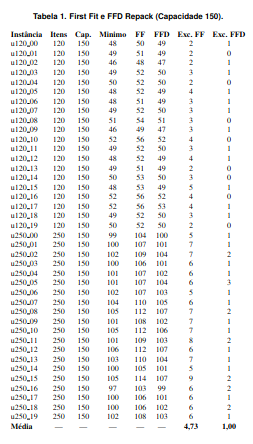
\includegraphics[width=0.7\textwidth]{table-ff.png}

O FFD Repack reduziu o excesso médio de 4,73 para 1,00 bin,
representando uma redução de aproximadamente 78,8\%. Em 8 das 20
instâncias da família \texttt{u120} (u120\_01, u120\_04, u120\_08,
u120\_10, u120\_13, u120\_14, u120\_16 e u120\_19), o algoritmo
atingiu o minimo  conhecido.

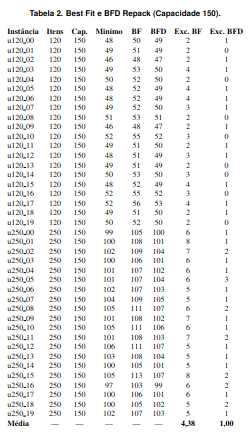
\includegraphics[width=0.7\textwidth]{table-bf.png}

O BFD Repack apresentou excesso médio de 1,00 bin, igual ao observado
para o FFD Repack, com redução de 77,1\% sobre o Best Fit. Esse
resultado sugere que, para a capacidade 150, o remanejamento contribui
para aproximar as soluções do minimo  conhecido,
independentemente da estratégia de encaixe inicial.

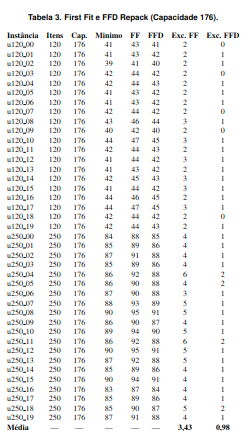
\includegraphics[width=0.7\textwidth]{table-ff-176.png}

Para a capacidade 176, o FFD Repack apresentou excesso médio de
0,98 bin, contra 3,43 do First Fit, o que corresponde a uma redução
de aproximadamente 71,5\%. Em 5 das 20 instâncias da família
\texttt{u120} (u120\_00, u120\_03, u120\_07, u120\_09 e u120\_18), o
algoritmo atingiu o mínimo de bins. Apesar do bom desempenho, o
excesso médio permaneceu ligeiramente superior ao observado para a
capacidade 150 (1,00 contra 0,98 bin), enquanto o gap relativo subiu
de 1,33\% para 1,52\%.

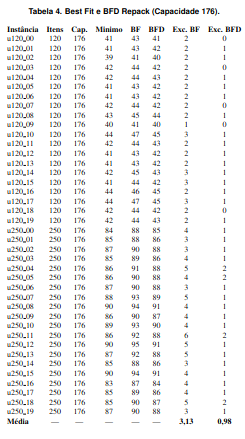
\includegraphics[width=0.7\textwidth]{table-bf-176.png}

Na capacidade 176, o BFD Repack apresentou excesso médio de 0,98 bin,
contra 3,13 do Best Fit, com redução de aproximadamente 68,8\%. Os
resultados são idênticos aos do FFD Repack em todas as instâncias,
confirmando o comportamento observado na capacidade 150: a etapa de
remanejamento domina o efeito da ordenação inicial, e ambos os
algoritmos com remanejamento convergem para as mesmas soluções.

\subsection{Resultados dos Algoritmos Exatos}

A seguir, são apresentados os resultados dos algoritmos exatos, começando pelo Branch and Bound e, em seguida, pelo Las Vegas.

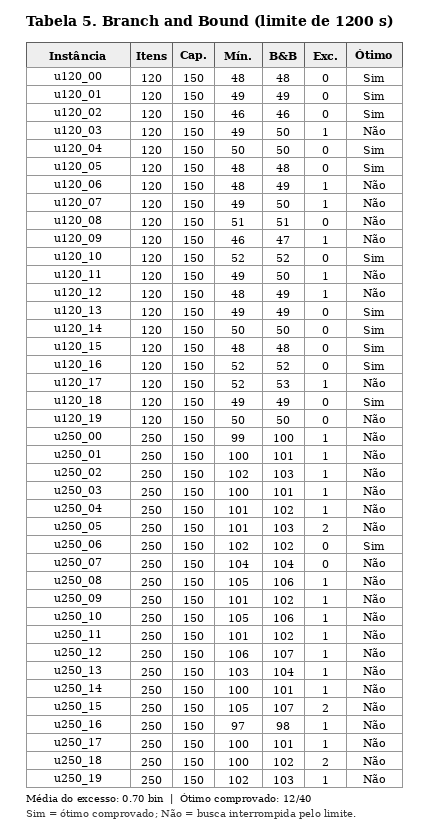
\includegraphics[width=0.7\textwidth]{table-branch-and-bound-20min.png}

Com limite de 1200 segundos por instância, o Branch and Bound comprovou a otimalidade em 12 dos 40 casos: 11 da família \texttt{u120} e a instância \texttt{u250\_06}. Nas outras 28 instâncias, a busca foi interrompida pelo limite de tempo.

O excesso médio em relação à melhor solução conhecida foi de 0,70 bin. Em três instâncias interrompidas (\texttt{u120\_08}, \texttt{u120\_19} e \texttt{u250\_07}), o algoritmo encontrou uma solução com o mesmo número de bins da melhor conhecida, embora não tenha comprovado a otimalidade. Nas outras 25 instâncias interrompidas, o excesso foi de um ou dois bins.

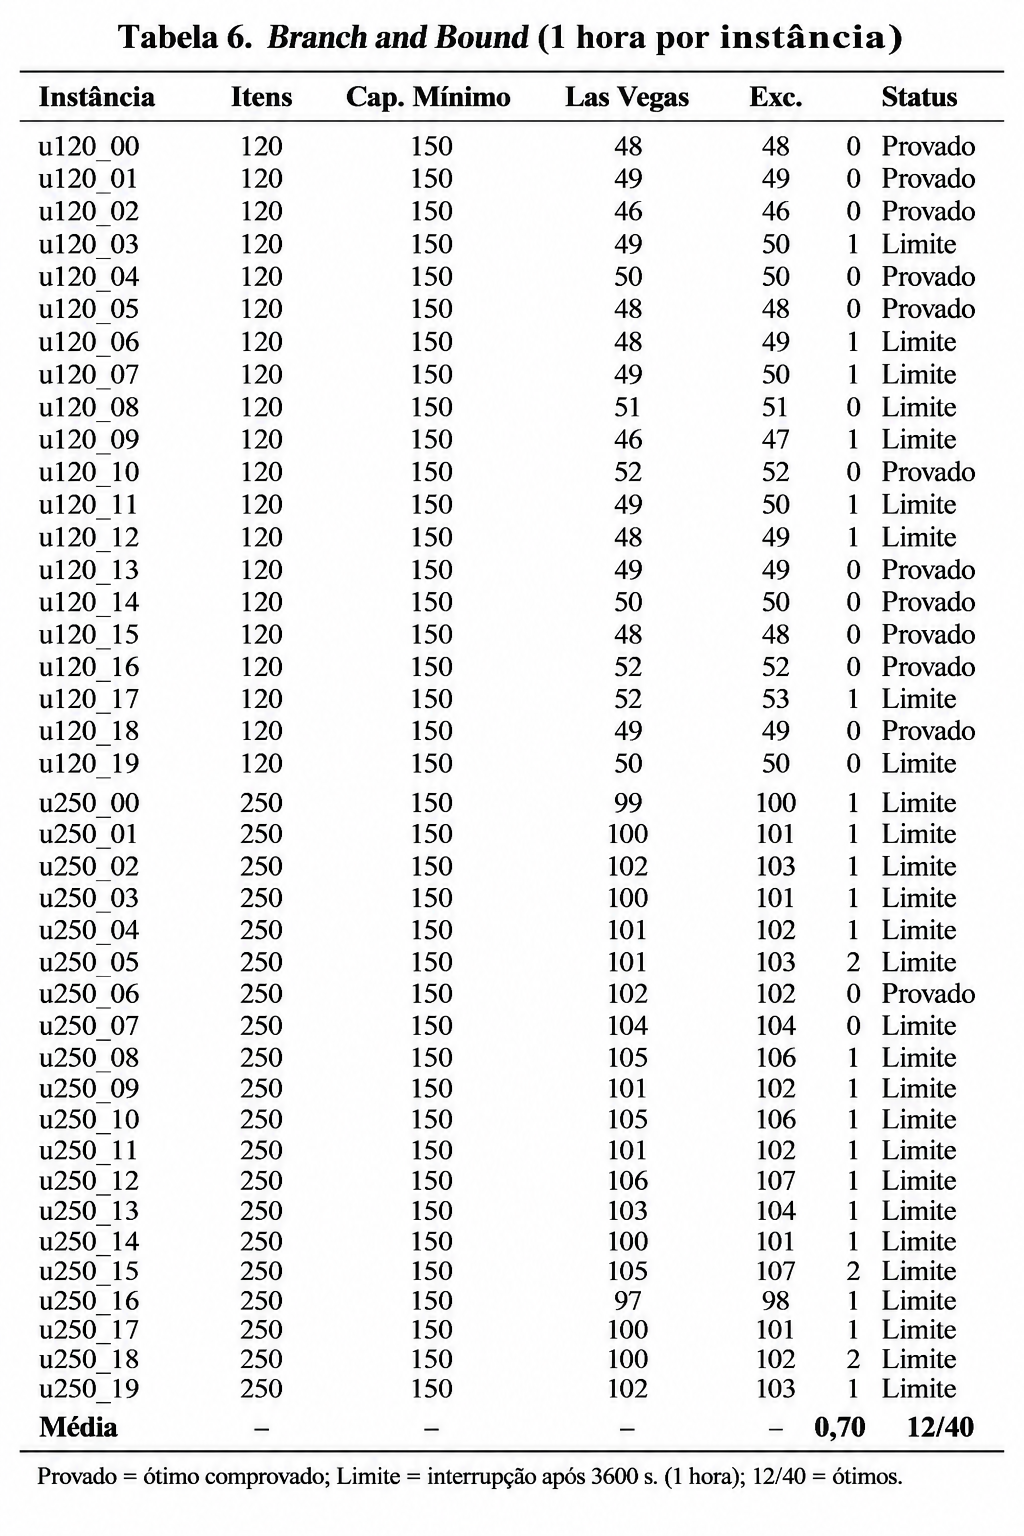
\includegraphics[width=0.7\textwidth]{table-branch-and-bound-1h.png}

Com o limite ampliado para 3600 segundos por instância, o Branch and Bound manteve os mesmos resultados: comprovou a otimalidade em 12 casos, enquanto as outras 28 buscas foram interrompidas. O excesso médio também permaneceu em 0,70 bin. Assim, nessa execução, o tempo adicional não alterou o número de bins encontrado nem aumentou a quantidade de instâncias com ótimo comprovado.

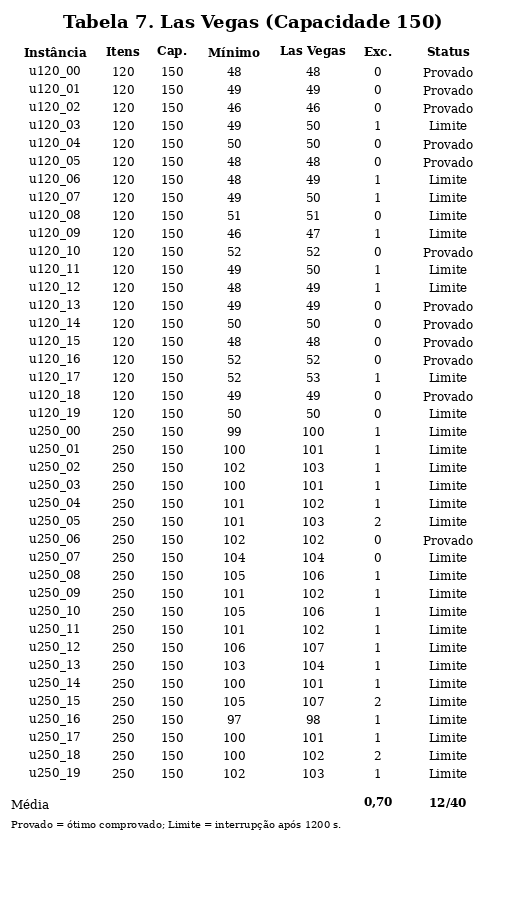
\includegraphics[width=0.7\textwidth]{table-las-vegas.png}

Já o Las Vegas, com tempo limite de 1200 segundos, apresentou os mesmos resultados do Branch and Bound de 20 minutos em número de bins e comprovação da otimalidade: 12 ótimos comprovados e 28 buscas interrompidas. O excesso médio também foi de 0,70 bin.

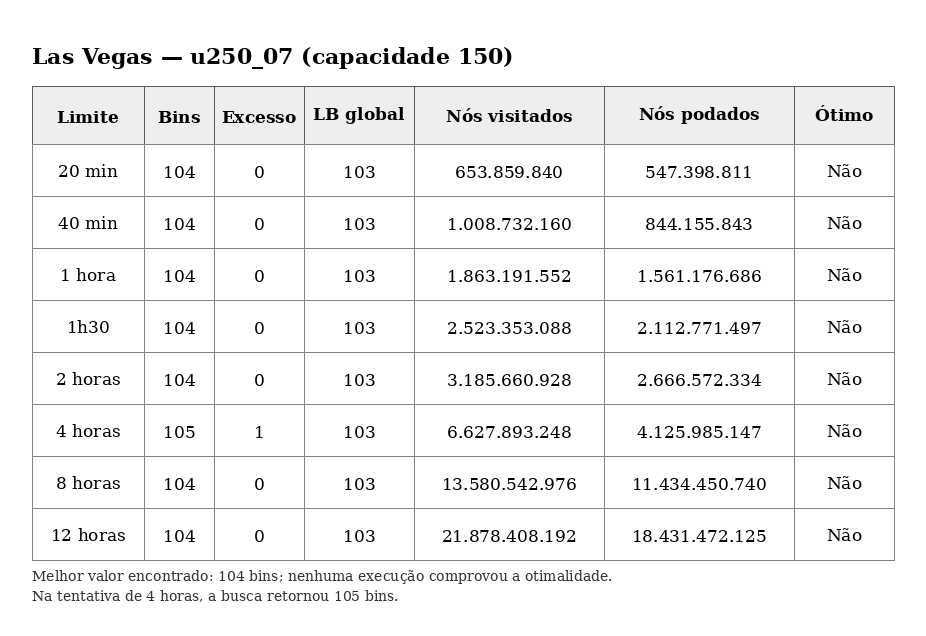
\includegraphics[width=0.7\textwidth]{table-las-vegas-u250-07-progressivo.png}

Para observar a variação entre os caminhos aleatorizados, a instância \texttt{u250\_07} foi executada separadamente com limites crescentes, de 20 minutos a 12 horas. Cada tentativa foi uma execução independente, com uma nova semente aleatória. Em sete das oito execuções, o algoritmo encontrou 104 bins, igual à melhor solução conhecida (mas não comprovou a otimalidade). No entanto, na tentativa de 4 horas, encontrou 105 bins. Essa diferença mostra que as execuções percorreram caminhos distintos e chegaram a soluções viáveis de qualidades diferentes.

Mesmo na execução de 12 horas, a otimalidade não foi comprovada: foram encontrados 104 bins, mas o limite inferior global permaneceu em 103. Portanto, o resultado coincide com a melhor solução conhecida, mas ainda não permite afirmar que ela seja ótima.

\section{Conclusão}

\subsection{Conclusão das Heurísticas}

Entre as heurísticas, FFD Repack e BFD Repack apresentaram os melhores resultados médios e encontraram soluções idênticas nas 40 instâncias, tanto na capacidade 150 quanto na capacidade 176. O excesso médio foi de 1,00 bin na capacidade 150 e de 0,98 na capacidade 176. Apesar de a capacidade 176 reduzir de 3017 para 2566 o total de bins da melhor solução conhecida, o gap relativo dos algoritmos com remanejamento aumentou de 1,33\% para 1,52\%. Além disso, nenhuma instância da família \texttt{u250} atingiu a melhor solução conhecida nas configurações testadas.

\subsection{Conclusão dos Algoritmos Exatos}

Com limite de 20 minutos, Branch and Bound e Las Vegas apresentaram os mesmos resultados: comprovaram a otimalidade em 12 das 40 instâncias e tiveram excesso médio de 0,70 bin. O Branch and Bound manteve esses resultados com o limite de 1 hora. Nas outras 28 instâncias, a busca foi interrompida pelo limite de tempo.

Os testes progressivos do Las Vegas na instância \texttt{u250\_07} também não comprovaram a otimalidade, mesmo com 12 horas. Em sete das oito execuções, foram encontrados 104 bins; na execução de 4 horas, foram encontrados 105. Como cada tentativa usou uma semente diferente, os caminhos percorridos e as melhores soluções viáveis variaram. O limite inferior global permaneceu em 103 bins, portanto não foi possível comprovar que a solução de 104 bins era ótima.

\subsection{Comparação entre Heurísticas e Métodos Exatos}

Na capacidade 150, os métodos exatos tiveram excesso médio de 0,70 bin, abaixo do excesso de 1,00 bin das heurísticas com remanejamento, 4,73 do First Fit e 4,38 do Best Fit. Por instância, Branch and Bound e Las Vegas encontraram soluções melhores que as heurísticas com remanejamento em 12 casos e iguais nas outras 28.

Embora os métodos exatos tenham encontrado soluções com o mesmo número de bins da melhor solução conhecida em 15 instâncias, comprovaram a otimalidade em apenas 12. Nas outras três, a busca foi interrompida pelo limite de tempo. Assim, os resultados indicam que os métodos exatos melhoraram a qualidade média das soluções na capacidade 150, mas nem sempre tiveram tempo para provar que eram ótimas. Para a capacidade 176, como os métodos exatos não foram executados, a comparação ficou restrita às heurísticas.

\bibliographystyle{sbc}
\bibliography{referencias}

\end{document}
